\documentclass[draft]{phd}

\begin{document}
	%
	\chapter*{Introduction}
	%
		%
The major success of theoretical physics in the last half century is certainly the unification of the electromagnetic, strong and weak forces in the framework of the Standard Model.
This is is based on \emph{Quantum Field Theory} -- a framework where local excitations interact according to the laws of quantum mechanics and special relativity -- and is, 
as far as we know, the most complete, experimentally verifiable theory of fundamental interactions. 
%
%		The main open problem in theoretical physics in the last half century is certainly the description of the four fundamental forces in a single unified framework.
%		So far we have witnessed impressive progresses for the last three interactions. 
%		We have a theory that describes them in quite a satisfactory way, even if several points remain obscure. 
	
What still remains an open question is how to include gravity in this picture, and this is due to the lack of renormalizability of the theory. 
%		This theory makes use of the \emph{Quantum Field Theory} -- a framework where local excitations interact according to the laws of quantum mechanics and special relativity -- and is commonly known as the \emph{Standard Model}. 
%		It is, as far as we know, the most complete, experimentally verifiable theory of fundamental interactions. 
%		Currently, the Standard Model is the agreed picture of fundamental physics among the physicists, also thanks to the important results from \textsc{CERN} and from many other laboratories. 
%		It has the important property of being \emph{renormalisable}. 
%		Indeed, some infinite quantities appear in calculating, for instance, correlators with perturbative methods. 
%		This problem afflicted many of the most brilliant minds of the last century, since correlation functions are related to observable quantities, that, of course, cannot be divergent. 
%		\emph{Renormalisation} is the procedure that removes these divergencies.
%		
%In what follows, we will focus on the so-called ultraviolet divergencies, since these are the relevant ones for the present discussion.
Usually a quantum field theory has ultra-violet divergencies that are cured by adding to the action a finite number of terms canceling the divergencies and such that the physical quantities do not depend on them. 
This procedure does not hold for Einstein gravity and, at present, there is no 
%
%may exist, but it is possible to introduce a finite set of, sometimes called, \emph{regularisation parameters}, such that physical quantities end up being finite. 
%		Then, renormalisation consists in the redefinition of the ``constants'' of the theory (mass, charge, etc.) through this set in such a way that the finite result is set-independent.
%		Obviously, there is a problem in this approach: it is not always applicable.
%		There are several conditions a theory must satisfy in order to be renormalisable, and Einstein's general relativity, the currently accepted theory of gravity, is not, furthermore there is not a full 
satisfactory way to quantize gravity.

Among the candidates 
%		The incompatibility of general relativity and quantum field theory is not only unsatisfactory from a theoretical perspective, but hampers the construction of a consistent theory of quantum gravity and the understanding of black holes.
%		Several extensions of Standard Model and brand new frameworks have been proposed in order to incorporate gravity into a quantum field description, but none of them can be confirmed by experiments yet. 
%		However, among the candidates 
for a quantum theory of gravity, string theory is perhaps the most promising one since, at least in principle, it also leads to unification of gravity and the other forces.

String theory is based on the simple but revolutionary idea of replacing, at the fundamental scale, point-like particles with one-dimensional extended objects -- the strings.
%This simple idea has a lot of very deep and still not completely understood and discovered implications, but the theory seems to be able to unify all forces of nature.
		
			%
				\begin{figure}[h]
					\centering
						\scalebox{.3}{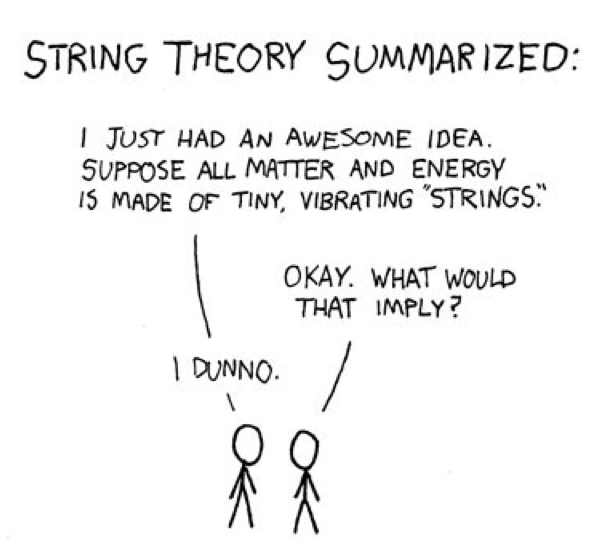
\includegraphics{./Resources/Images/Stringtheory.jpg}}
				\end{figure}
			%
The fundamental constituents of the universe are extremely tiny vibrating strings moving in spacetime. Strings can have the topology of a segment -- open strings -- 
 or that of a circle -- closed strings.
 %		These objects can appear in two different topologies, the segment and the circle, \emph{i.e.} we can have open and closed strings.
%		For each of these topologies, 
%	
	
The quantised string has a discrete spectrum of vibration modes, which at large distances (much larger than the characteristic string length $\ell_s = \sqrt{\alpha'}$) can be effectively
interpreted as different point particles. 
The spectrum contains a finite number of massless states and infinite tower of massive states with masses of order $1/\sqrt{\alpha'}$.
The theory was invented in another context (to describe strong interactions), but it came back to glory when it was realised that in the spectrum of the closed string there is always a massless spin 2 mode. One can identify it with the graviton, and therefore string theory automatically incorporates gravity. Since, among the massless states there can also be
gauge bosons, string theory provides a framework for the unification of all fundamental forces, that reproduces, as low energy limit, Einstein theory and gauge theories.


		
The short distance singularities are avoided due to the extended nature of the string. A string sweeps a two-dimensional surface -- the world-sheet -- that is a smooth manifold and the interaction vertices are given by diagrams as in~\cref{stringdiagram}.
			%
				\begin{figure}[ht]
					\centering
						\scalebox{1.3}{\documentclass[border=5mm,tikz]{standalone}

\usepackage{amsmath, amssymb, amsfonts, amscd, amsthm, bigints, units}
%!TEX encoding = UTF-8 Unicode
\usepackage{tikz}
\usepackage{tikz-cd}
\usepackage{tikz3dcs-pp}
\usepackage{pgfplots}
\usepackage{xcolor, eecolors}
\usepackage{math, lrmath}

\usepackage{pgfplots}
\usepgfplotslibrary{patchplots}
\pgfplotsset{compat=1.15}

\usetikzlibrary{calc, intersections}

\usetikzlibrary{decorations.pathmorphing,calc,shapes,positioning,fit,arrows,fadings,decorations.pathreplacing,decorations.pathmorphing,intersections,patterns, trees}
\usetikzlibrary{decorations.markings}

\usepackage{marvosym}

%%%%%%%%My Tikz definitions%%%%%%%%%%%%%%%%%
\tikzset{->-/.style={decoration={
  markings,
  mark=at position #1 with {\arrow{latex}}},postaction={decorate}}}
  %
\tikzset{
    %Define standard arrow tip
    >=stealth',
    %Define style for boxes
    punkt/.style={
           rectangle,
           rounded corners,
           draw=black, very thick,
           text width=7.5em,
           minimum height=2em,
           text centered},
    % Define arrow style
    pil/.style={
           ->,
           thick,
           shorten <=2pt,
           shorten >=2pt,}
}
%%%
%%3d drawings %%%
\newcommand\pgfmathsinandcos[3]{%
  \pgfmathsetmacro#1{sin(#3)}%
  \pgfmathsetmacro#2{cos(#3)}%
}
\newcommand\LongitudePlane[3][current plane]{%
  \pgfmathsinandcos\sinEl\cosEl{#2} % elevation
  \pgfmathsinandcos\sint\cost{#3} % azimuth
  \tikzset{#1/.style={cm={\cost,\sint*\sinEl,0,\cosEl,(0,0)}}}
}
\newcommand\LatitudePlane[3][current plane]{%
  \pgfmathsinandcos\sinEl\cosEl{#2} % elevation
  \pgfmathsinandcos\sint\cost{#3} % latitude
  \pgfmathsetmacro\yshift{\cosEl*\sint}
  \tikzset{#1/.style={cm={\cost,0,0,\cost*\sinEl,(0,\yshift)}}} %
}
\newcommand\DrawLongitudeCircle[2][1]{
  \LongitudePlane{\angEl}{#2}
  \tikzset{current plane/.prefix style={scale=#1}}
   % angle of "visibility"
  \pgfmathsetmacro\angVis{atan(sin(#2)*cos(\angEl)/sin(\angEl))} %
  \draw[current plane] (\angVis:1) arc (\angVis:\angVis+180:1);
  \draw[current plane,dashed] (\angVis-180:1) arc (\angVis-180:\angVis:1);
}
\newcommand\DrawLatitudeCircle[2][1]{
  \LatitudePlane{\angEl}{#2}
  \tikzset{current plane/.prefix style={scale=#1}}
  \pgfmathsetmacro\sinVis{sin(#2)/cos(#2)*sin(\angEl)/cos(\angEl)}
  % angle of "visibility"
  \pgfmathsetmacro\angVis{asin(min(1,max(\sinVis,-1)))}
  \draw[current plane] (\angVis:1) arc (\angVis:-\angVis-180:1);
  \draw[current plane,dashed] (180-\angVis:1) arc (180-\angVis:\angVis:1);
}
%%%%


\begin{document}

	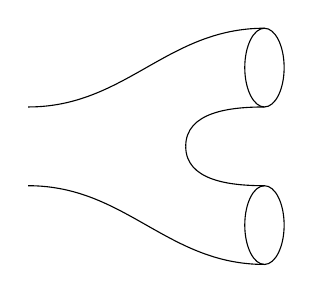
\begin{tikzpicture}[rotate=90]
		  \def\R{0.5}
		  \def\angEl{-30}
			   \DrawLatitudeCircle[\R]{0}
			  %\draw[dashed] (0,.5) arc (0:180: .5 and .25);
			  %\draw (0,.5) arc (180:360: .5 and .25);
			  \draw (-1,-3) ellipse (.5 and .25);
			  \draw (1,-3) ellipse (.5 and .25);
			  \draw (-.5,0) to[out=-90,in=90] (-1.5,-3);
			  \draw (.5,0) to[out=-90,in=90] (1.5,-3);
			  \draw (-.5,-3) to[out=90,in=180] (0,-2);
			  \draw (0,-2) to[out=0,in=90] (.5,-3);
	\end{tikzpicture}

\end{document}
}
					\caption{Feynman diagram of a string interaction vertex. 
						Imposing the finite dimension of the fundamental objects, we lose the \emph{locality} of the interactions, but we can cure the short-distance divergences.
						Now, Feynman diagrams are smooth $2$-dimensional surfaces and the interaction vertices have been ``smoothed out''.
					 }
					\label{stringdiagram}
				\end{figure}
			%
This provides an ultraviolet regularisation of the graviton scattering amplitudes, whose divergence was due to the point-wise nature of the interaction.
		
Generically the string spectrum contains 
%		From a formal point of view, the only parameter in the theory that is needed to be measured is $\alpha'$, connected to the string length.
%		The quantisation of the string motion imposes further constraints, \emph{e.g.} the spectrum of the bosonic string\footnote{%
%			A string theory where only bosonic modes are allowed.}
tachyons, which can be interpreted as instabilities of the space-time.
These can be avoided by imposing that the spectrum is supersymmetry and gives rise to \emph{superstring theory}. \\
The evolution of the string is described by a two-dimensional conformal field theory defined on its world-sheet. 
To keep conformal invariance at the quantum level 
%		We want to preserve this world-sheet symmetry even after the quantisation procedure. The conditions to have Weyl anomaly\footnote{%
%			An \emph{anomaly} is a quantum effect breaking a classical symmetry. The Weyl anomaly is the anomaly breaking the conformal symmetry.}
%		cancellation 
constrains the space-time where the string leaves to be ten-dimensional. \\
Taking into account all the constraints and consistency conditions, it turns out that there are only five possible superstring theories: type I, type IIA, type IIB and the two heterotic theories $\SO(32)$ and $\E_8 \times \E_8$, which have different field contents. 
In all these cases, it is possible to derive an effective quantum field theory for the massless states: these are called supergravity theories since they contain gravity and are
supersymmetric. Supergravity theories have been discovered independently from string theory in the mid seventies, 
and only later stage it was realised that they corresponded to the low energy limit of string theory.
Notice also that all supergravity theories are non renormalizable, but they make sense as effective theories of the string. \\
As we will discuss in detail later, a common feature of all ten-dimensional supergravity theories is the presence of higher-rank gauge fields -- the NS and RR fields -- 
which played a major role in all recent developments of string theory.


In mid 1990s the discovery of string dualities allowed to show that superstring theories are actually different formulations of the same theory, which are valid
in different corners of the parameter space and are related to more fundamental theory, which is conjectured to live in eleven spacetime dimensions, and has been given the name of M-theory.\footnote{%
			We know the $11$-dimensional supergravity, so the corresponding high energy fundamental theory is identified with M-theory.
			We do not have a complete formulation of M-theory yet, but we know the degrees of freedom of the theory.
			This tells us that the fundamental dynamical ingredients of this theory are not strings, but higher dimensional objects: branes.
			We are going back to branes in the following.}.	\\
The net of dualities involve other fundamental dynamical objects, besides strings, called branes. A Dp-brane is a solitonic entended\footnote{It has a (p+1)-dimensional world volume.} object that is charged under one 
of the NS and RR potentials, generalising the coupling of charged particle to the electric field. Crucially for many applications, in string theory, a 
 D-brane also has a perturbative description as dynamical hyperplanes on which open strings can end.\footnote{More precisely a Dp-brane is an open string with $p+1$ \emph{Dirichelet} boundary conditions.}
				%
					\begin{figure}[h!]
						\centering
						\documentclass[border=2pt]{standalone}

\usepackage{amsmath, amssymb, amsfonts, amscd, amsthm, bigints, units}
%!TEX encoding = UTF-8 Unicode
\usepackage{tikz}
\usepackage{tikz-cd}
\usepackage{tikz3dcs-pp}
\usepackage{pgfplots}
\usepackage{xcolor, eecolors}
\usepackage{math, lrmath}

\usepackage{pgfplots}
\usepgfplotslibrary{patchplots}
\pgfplotsset{compat=1.15}

\usetikzlibrary{calc, intersections}

\usetikzlibrary{decorations.pathmorphing,calc,shapes,positioning,fit,arrows,fadings,decorations.pathreplacing,decorations.pathmorphing,intersections,patterns, trees}
\usetikzlibrary{decorations.markings}

\usepackage{marvosym}

%%%%%%%%My Tikz definitions%%%%%%%%%%%%%%%%%
\tikzset{->-/.style={decoration={
  markings,
  mark=at position #1 with {\arrow{latex}}},postaction={decorate}}}
  %
\tikzset{
    %Define standard arrow tip
    >=stealth',
    %Define style for boxes
    punkt/.style={
           rectangle,
           rounded corners,
           draw=black, very thick,
           text width=7.5em,
           minimum height=2em,
           text centered},
    % Define arrow style
    pil/.style={
           ->,
           thick,
           shorten <=2pt,
           shorten >=2pt,}
}
%%%
%%3d drawings %%%
\newcommand\pgfmathsinandcos[3]{%
  \pgfmathsetmacro#1{sin(#3)}%
  \pgfmathsetmacro#2{cos(#3)}%
}
\newcommand\LongitudePlane[3][current plane]{%
  \pgfmathsinandcos\sinEl\cosEl{#2} % elevation
  \pgfmathsinandcos\sint\cost{#3} % azimuth
  \tikzset{#1/.style={cm={\cost,\sint*\sinEl,0,\cosEl,(0,0)}}}
}
\newcommand\LatitudePlane[3][current plane]{%
  \pgfmathsinandcos\sinEl\cosEl{#2} % elevation
  \pgfmathsinandcos\sint\cost{#3} % latitude
  \pgfmathsetmacro\yshift{\cosEl*\sint}
  \tikzset{#1/.style={cm={\cost,0,0,\cost*\sinEl,(0,\yshift)}}} %
}
\newcommand\DrawLongitudeCircle[2][1]{
  \LongitudePlane{\angEl}{#2}
  \tikzset{current plane/.prefix style={scale=#1}}
   % angle of "visibility"
  \pgfmathsetmacro\angVis{atan(sin(#2)*cos(\angEl)/sin(\angEl))} %
  \draw[current plane] (\angVis:1) arc (\angVis:\angVis+180:1);
  \draw[current plane,dashed] (\angVis-180:1) arc (\angVis-180:\angVis:1);
}
\newcommand\DrawLatitudeCircle[2][1]{
  \LatitudePlane{\angEl}{#2}
  \tikzset{current plane/.prefix style={scale=#1}}
  \pgfmathsetmacro\sinVis{sin(#2)/cos(#2)*sin(\angEl)/cos(\angEl)}
  % angle of "visibility"
  \pgfmathsetmacro\angVis{asin(min(1,max(\sinVis,-1)))}
  \draw[current plane] (\angVis:1) arc (\angVis:-\angVis-180:1);
  \draw[current plane,dashed] (180-\angVis:1) arc (180-\angVis:\angVis:1);
}
%%%%


\begin{document}

	\begin{tikzpicture}
	%
		\draw[name path=braneA, smooth cycle, tension=0, fill=white, pattern color=orange, pattern=north west lines, opacity=.5] plot coordinates{(-5,2) (-6,0) (-6,-5) (-5,-3)};
		
		\draw[name path=braneB, smooth cycle, tension=0, fill=white, pattern color=blue, pattern=north west lines, opacity=.5] plot coordinates{(0,2) (-1,0) (-1,-5) (0,-3)};
		
		\draw [name path=openString, thick, red] (-5.3, 0) to[out=45, in = 210] (-1, -.5);
		\draw [name path=openString, thick, dashed, red] (-1, -.5) to[out=30, in = 190] (-.3, 0);
		
		\draw [color = green, smooth, tension=1, thick] plot coordinates{(-5.7, -1.5) (-4.7, -1) (-4.5, -2) (-4, -2.9)  (-5.7, -3.3)};

	%
	\end{tikzpicture}

\end{document}

						\caption{Branes are hypersurface where open strings (or other branes) can end.}
						\label{branefig}
					\end{figure}
				%
%			Recall that a $\mathrm{D}_p$ brane is a $(p+1)$-dimensional object, with $p$ spatial dimensions.
%			Analysing the structure of the brane action~\cite{PolchinskiBranes}, one can see that on the brane always couples to a $p+1$-form potential $C_{p+1}$, through a term that schematically looks like,
%				%
%					\begin{equation*}
%						\mu \int_{\Sigma} C_{p+1}\, ,
%					\end{equation*}
%				%
%			where $\mu$ is the charge of the brane and $\Sigma$ its world-volume.
%			One can measure the electric and magnetic charges of the branes integrating the field strength,
%				%
%					\begin{align*}
%						& & q = \!\!\!\!\! \int\displaylimits_{S^{D-p-2}} \star F_{p+2} \, , & & p = \!\!\!\!\! \int\displaylimits_{S^{D-p-2}} F_{p+2} \, , & &
%					\end{align*}
%				%
%			where we denoted by $S^{D-p-2}$ the infinite radius sphere surrounding the brane in $D$ dimensions.
%			Then it is easy to see that each $\mathrm{D}_p$ brane couples electrically and magnetically to $p+2$- and $(D-p-2)$-form field strengths.
%			This is actually true also for other kinds of branes, \emph{i.e.} those which are not hypersurfaces where strings can end, but still they are dynamical objects in the theory.
%			For instance, in M-theory there are no strings, so branes in this theory are not D-branes, we call them M-branes.
			
			Because of the different spectra, each theory has its own stable branes. In M-theory there are M$2$ and M$5$ branes.
Type IIA has $\mathrm{D}_p$ branes with $p$ even, while Type IIB has $\mathrm{D}_p$ branes with $p$ odd.
Further, both type II string theories share a brane that couples electrically with the $2$-form Kalb-Ramond potential $B$, 
a $5$-brane usually called NS$5$ brane.
Branes are dynamical objects whose dynamic is governed by the fields that leaves on their world-volume. This is a very important property that lead to
the discovery of the AdS/CFT correspondence and all its developments.

			
%			Moreover, branes have fields that only exist on their world-volume and not in the embedding space\footnote{%
%				This is the basic reason for another explanation of the extra-dimensions, \emph{i.e.} the so-called \emph{brane world scenario}.
%				This idea states that we live actually on a D$_3$ brane, embedded in a $10$-dimensional string background.
%				We are not going to analyse further this interesting topic. 
%				We refer to a nice review~\cite{BraneWorldCosmo} and references therein.%
%			},
%			see~\cref{braneworld}.
%				%
%					\begin{figure}[h!]
%						\centering
%						\scalebox{.7}{\documentclass[border=2pt]{standalone}

\usepackage{amsmath, amssymb, amsfonts, amscd, amsthm, bigints, units}
%!TEX encoding = UTF-8 Unicode
\usepackage{tikz}
\usepackage{tikz-cd}
\usepackage{tikz3dcs-pp}
\usepackage{pgfplots}
\usepackage{xcolor, eecolors}
\usepackage{math, lrmath}

\usepackage{pgfplots}
\usepgfplotslibrary{patchplots}
\pgfplotsset{compat=1.15}

\usetikzlibrary{calc, intersections}

\usetikzlibrary{decorations.pathmorphing,calc,shapes,positioning,fit,arrows,fadings,decorations.pathreplacing,decorations.pathmorphing,intersections,patterns, trees}
\usetikzlibrary{decorations.markings}

\usepackage{marvosym}

%%%%%%%%My Tikz definitions%%%%%%%%%%%%%%%%%
\tikzset{->-/.style={decoration={
  markings,
  mark=at position #1 with {\arrow{latex}}},postaction={decorate}}}
  %
\tikzset{
    %Define standard arrow tip
    >=stealth',
    %Define style for boxes
    punkt/.style={
           rectangle,
           rounded corners,
           draw=black, very thick,
           text width=7.5em,
           minimum height=2em,
           text centered},
    % Define arrow style
    pil/.style={
           ->,
           thick,
           shorten <=2pt,
           shorten >=2pt,}
}
%%%
%%3d drawings %%%
\newcommand\pgfmathsinandcos[3]{%
  \pgfmathsetmacro#1{sin(#3)}%
  \pgfmathsetmacro#2{cos(#3)}%
}
\newcommand\LongitudePlane[3][current plane]{%
  \pgfmathsinandcos\sinEl\cosEl{#2} % elevation
  \pgfmathsinandcos\sint\cost{#3} % azimuth
  \tikzset{#1/.style={cm={\cost,\sint*\sinEl,0,\cosEl,(0,0)}}}
}
\newcommand\LatitudePlane[3][current plane]{%
  \pgfmathsinandcos\sinEl\cosEl{#2} % elevation
  \pgfmathsinandcos\sint\cost{#3} % latitude
  \pgfmathsetmacro\yshift{\cosEl*\sint}
  \tikzset{#1/.style={cm={\cost,0,0,\cost*\sinEl,(0,\yshift)}}} %
}
\newcommand\DrawLongitudeCircle[2][1]{
  \LongitudePlane{\angEl}{#2}
  \tikzset{current plane/.prefix style={scale=#1}}
   % angle of "visibility"
  \pgfmathsetmacro\angVis{atan(sin(#2)*cos(\angEl)/sin(\angEl))} %
  \draw[current plane] (\angVis:1) arc (\angVis:\angVis+180:1);
  \draw[current plane,dashed] (\angVis-180:1) arc (\angVis-180:\angVis:1);
}
\newcommand\DrawLatitudeCircle[2][1]{
  \LatitudePlane{\angEl}{#2}
  \tikzset{current plane/.prefix style={scale=#1}}
  \pgfmathsetmacro\sinVis{sin(#2)/cos(#2)*sin(\angEl)/cos(\angEl)}
  % angle of "visibility"
  \pgfmathsetmacro\angVis{asin(min(1,max(\sinVis,-1)))}
  \draw[current plane] (\angVis:1) arc (\angVis:-\angVis-180:1);
  \draw[current plane,dashed] (180-\angVis:1) arc (180-\angVis:\angVis:1);
}
%%%%


\begin{document}

% Define styles for the different kind of edges in a Feynman diagram
\tikzset{
    photon/.style={decorate, decoration={snake}, draw=red},
    electron/.style={draw=blue, postaction={decorate},
        decoration={markings,mark=at position .55 with {\arrow[draw=blue]{>}}}},
    antielectron/.style={draw=blue, postaction={decorate},
        decoration={markings,mark=at position .55 with {\arrow[draw=blue]{<}}}},
    gluon/.style={decorate, draw=magenta,
        decoration={coil,amplitude=4pt, segment length=5pt}} 
}

\begin{tikzpicture}[
        thick,
        % Set the overall layout of the tree
        level/.style={level distance=1.5cm},
        level 2/.style={sibling distance=2.6cm},
        level 3/.style={sibling distance=2cm}
    ]
    \coordinate
        child[grow=left]{
            child {
                node {}
                % The 'edge from parent' is actually not needed because it is
                % implicitly added.
                edge from parent [antielectron]
            }
            child {
                node {}
                edge from parent [antielectron]
            }
            edge from parent [photon] node{}
        }
        % I have to insert a dummy child to get the tree to grow
        % correctly to the right.
        child[grow=right, level distance=0pt] {
        child  {
	edge from parent [electron]
            node [below] {}
        }
        child {
            edge from parent [electron]
            node [above] {}
        }
    };
    
     \begin{scope}[xscale=3, yscale = 2]
	\draw[name path=braneA, smooth cycle, tension=0, fill=white, pattern color=orange, pattern=north west lines, opacity=.3] plot coordinates{(1.5,3) (-1.5,2) (-1.5,-2) (1.5,-1)};
	\draw [name path=openString, red] (-1.5, 2.1) to[out=0, in = 170] (-.7, 2.25);
	\draw [name path=openString, dashed, red] (-.7, 2.25) to[out=-20, in = 190] (1, 2.2);
	\draw [green, fill = green ] (1,2.2) circle (.01)
		node[black] at (.8, 2.07) {$p$}
		node[black] at (1.2,.3) {\Huge \Gentsroom \Ladiesroom};
	\draw [->, green, thick] (1,2.2) -- (1, 1.7);
	\draw [->, green, thick] (1,2.2) -- (1.2, 1.8);
	\draw [->, green, thick] (1,2.2) -- (1.3, 2.3);
	\draw [->, green, thick] (1,2.2) -- (1, 2.7);
	\draw [->, green, thick] (1,2.2) -- (1.2, 2.5);
	\draw [->, green, thick] (1,2.2) -- (.8, 2.5);
	\draw [->, green, thick] (1,2.2) -- (.85, 1.85);
	\draw [->, green, thick] (1,2.2) -- (1.25, 2.07);
     \end{scope}
\end{tikzpicture}


\end{document}
}
%						\caption{Branes have fields living only on their world-volume (here the point $p$ is a source for the observers on the brane).
%							Brane World scenario sees our universe as living on a D$_3$ brane.}
%						\label{braneworld}
%					\end{figure}
%				%
%			Often, in supergravity, one refers to branes just by $p$-branes, denoting their spatial dimension, but not their stringy origin, that is we can indicate with $5$-brane both an M$5$ or a D$_5$ when we are not worried to add any further distinction.
%

%
%		
%		As mentioned above, at low energies strings might be considered as particles. 
%		The theory coming out of the particle limit of string theory is \emph{supergravity}.
%		As the name may suggest, \emph{supergravity} is a theory encoding both Einstein gravity and supersymmetry (making this a point-wise symmetry).
%		It was discovered independently from string theory in mid seventies, and only at a later stage physicists realised it was a limit at low energy scales of the latter.
		
		The introduction one-dimensional elementary objects seems to solve the conflict between general relativity and quantum field theory and to provide a framework for the unification of all fundamental forces.
		However, we pay a price. Space-time has extra-dimensions.
		This is one of the most striking predictions of string theory, and a model based on this framework with some hope to describe nature has to cope with this issue.
		
		One option to face this concern is called \emph{compacification}.
		It consists in assuming the original spacetime to have four large non-compact spacetime directions -- the ones we have experience of -- while the remaining ones are instead wrapped on themselves to form a very tiny compact space.
		The characteristic dimension of this space is very small, such to explain why we do not have access to it (there are actually some bounds on the maximal length these dimensions can have. These bounds are being updated constantly due to on going measures at LHC, see for example~\cite{extradim1,extradim2}).
		More formally, we are interested in string solutions with a topology like,
			%
				\begin{equation*}
					\mathcal{M}_{10} = \mathcal{X}_4 \times M_6\, ,
				\end{equation*}
			%
		where $\mathcal{X}$ is the non-compact \emph{external spacetime}, and $M_d$ is the compact \emph{internal} manifold.
		Because of the small size of the extra-dimensions, the motion and excitation of the strings will look to us essentially four-dimensional. 
%		
%		In order to get an effective field theory in lower dimension, one has to integrate the higher dimensional theory over the internal manifold to get only external spacetime quantities.
However the external dimensions are not invisible: the features of the effective four-dimensional theory -- particle content, symmetries, masses, etc. -- 
depend on the geometry of the internal space.

Supersymmetry comes naturally in string theory, A major question is what amount of supersymmetry has the low-energy effective theory.
From a phenomenological point of view, the most desirable case is preserving a minimal amount of supersymmetry -- $\mathcal{N}=1$ -- since this allows for chiral fermions and it is 
compatible with the minimal extensions of the Standard Model.\footnote{% 
			The scale of susy breaking can tested in present day accelators. It is highly possible that the scale of susy breaking is much higher than what expected
			until now and this must be taken into account in string compactification models.}
A residual supersymmetry is welcome also for technical purposes, since it guarantees the stability of given string solutions and also allows for simpler ways of finding
string vacua.

What is very important for this thesis is that the conditions for a given string background to be supersymmetric 
 translate into topological and differential conditions on the internal manifold and strongly constrains its geometry.
 The best known example is the case purely geometric compactifications of string theory to four-dimensions, where the internal manifold is constrained to be 
 a Calabi-Yau three-fold, namely a $6$-dimensional manifold with $\SU(3)$ holonomy~\cite{CYcomp}.
The geometry of Calbi-Yau manifolds is well known and this makes it possible to explicitly compute the low-energy four-dimensional effective actions on these compactifications.
However the theories obtained this way are not good for phenomenology since they contain many massless scalar fields -- the moduli -- that are not constrained by any potential.

 A possible way to solve the moduli problem is to find a mechanism to generate a potential for them in the lower-dimensional action.
This would have the effect of stabilise the moduli (giving them a mass and a fixed vev).
A great number of results in this direction have been reached in the last twenty years, realising that it is possible to generate a non-trivial scalar potential 
considering more general string back-grounds where some of the RR and NS field take non-trivial expectation values. \emph{fluxes}~\cite{fluxcomp1, fluxcomp2, fluxcomp3}.
One can find some nice reviews of the subject in~\cite{DuffReviewComp, MarianaFluxReview, LustReviewComp, henlect}.
 However such fields back-react on the geometry and new tools are required to analyse and study the internal compactification manifolds, which are not Calabi-Yau.
 The methods described in this thesis are promising tools in this direction.
 
 Usually, a dimensionally reduced theory has an infinite number of states with higher dimensional origin.
 We are interested in constructing effective actions with a finite number of degrees of freedom, hence we have to give a prescription to \emph{truncate} out some of the modes.
 We call \emph{truncation ansatz} this prescription.
 Among all the possible truncation ansatze, a particular class is made by the ones having the property of being \emph{consistent}.
 A \emph{consistent truncation} is a choice of a finite set of modes, where the omitted ones are not sourced by the subset chosen. 
 This is equivalent to say that the set of truncated modes has a dynamics which is not affected by the others.
 We are interested in such truncations since any solution of the lower dimensional theory can be uplifted to a solution of the higher dimensional one.

		
		Reasons to study compactifications are not only phenomenological.
		There are important formal motivations.
		Many supergravity theories in various dimensions are connected by compactifications.
		Historically, since the birth of supergravity, dimensional reductions have been used to build lower dimensional models from the higher dimensional ones.		
		A first milestone example is the derivation of the four-dimensional maximally supersymmetric supergravity theory from the eleven-dimensional supergravity, due to Cremmer and Julia~\cite{CremmerJulia}.
		
%		We will see that the modern approach to model building via compactifications involves several ingredients. 
%		Among these there are localised objects like D- or M-branes, which typically are taken intersecting among them.
%		For various reasons, one is also led to add other tools like fluxes of the higher-dimensional fields and non-perturbative quantum effects. 
%		Clearly, it is very hard to have full control on all these ingredients at once, so that often one prefers to focus on certain aspects of the whole picture. 
%		In this thesis, we will focus on the relation between geometry and supersymmetry in compactifications, having a look also at supersymmetric conditions for branes.
%		
%		We are going to expose some facts about compactifications and geometry.
%		Further, we collect some notions about branes and their supersymmetric configurations, since this will be the matter of~\ref{chapbrane}. 


\subsection*{Outline of the thesis}
		%
		
			Extension of differential geometry turned out to be powerful tools to study generic string compactifications. 
			One of these is Generalised Geometry and the main goal of this thesis is to study its applications to various contexts in supergravity, principally consistent truncations and brane calibrations.
			The thesis is organised as follows.
			
			In the first two chapters we introduce the mathematical tools which are needed in the following.
			In particular, in chapter~\ref{chap1} are given the main definitions and examples of $G$-structures. 
			The concept of torsion of a structure is analysed and we show how the torsionless conditions for some structure are equivalent to reformulate the supersymmetry conditions on the manifold.
			Finally, we expose some facts about the special holonomy of a manifold.
			
			Chapter~\ref{chapSugra} is needed to give the physical environment we are moving in. 
			We briefly review the main features of the theories of supergravity we analyse in this thesis. 
			In addition we show how the $G$-structures can be fruitfully used to describe fluxless compactifications, but how they fail to capture all the informations in the presence of fluxes.
			
			Chapter~\ref{chapEGG} is based on the exposition of the main aspect of Generalised Geometry, both complex (useful as introduction) and exceptional.
			We will face the generalisation of the $G$-structures in this context and we will build an example of how flux compactifications are elegantly encoded in this formalism.
			In particular, an appealing feature of this approach is that one can predicts the lower-dimensional supergravity independently of many explicit computations.
			We will focus on maximally supersymmetric truncations, dealing with generalised parallelisation, that we will briefly review in~\ref{secGenPar}.
			
			The core of the thesis are chapters~\ref{chapComp} and~\ref{chapbrane}.
			The~\cref{chapComp} is about flux compactifications and consistent truncations. 
			In particular, we define generalised Scherk-Schwarz reductions, and we build a concrete example of truncations of massive IIA, building also an appropriate version of Exceptional Generalised Geometry adapted to it~\cite{oscar1}.
			
			On the other hand, the~\cref{chapbrane} is centered on branes and their calibrations.
			We study brane probes in AdS backgrounds (both in M-theory and type IIB) and we look for the supersymmetric configurations of these probes. It is a notorious fact that these corrispond to probes wrapping (generalised) calibrated submanifolds.
			Using the formalism of generalised geometry and $G$-structures we show how the integrability conditions on generalised HV structures~\cite{AshmoreESE} are equivalent to have supersymmetric branes in AdS backgrounds. 
			In other words, one can state that HV structures provide generalised calibrations of branes in such backgrounds.
			
			The thesis is completed by two appendices collecting conventions and technical remarks in exceptional generalised geometry.
			
			The core of this thesis is built on the following works
				%
					\begin{itemize}
						\item[] \cite{oscar1}~\bibentry{oscar1}
						\item[] \cite{oscar2}~\bibentry{oscar2}
					\end{itemize}
				%
			Other projects still in progress are
				%
					\begin{itemize}
						\item[] \cite{oscar3}~\bibentry{oscar3}
						\item[] \cite{oscar4}~\bibentry{oscar4}
						\item[] \cite{oscar5}~\bibentry{oscar5}
					\end{itemize}
				%			
		%
	%
\end{document}